\documentclass[a4paper,12pt,english]{all-in-one} %% TWOSIDE
\usepackage{amsmath} 
\usepackage{newtxmath}
\usepackage{multicol}
\usepackage{lipsum}
\usepackage{subfig}
\usepackage{listings}
\usepackage[hidelinks]{hyperref}
\renewcommand\theequation{\arabic{equation}}
\newcommand\tab[1][1cm]{\hspace*{#1}} 

\doctitle{Modern Physics Laboratory }
\docsubtitle{Hall effect} % Experiment name here

\makeatletter
\title{{\large\textit{Modern Physics Laboratory | PHYS-461}}\\[0.5cm]{\Huge\color{gray}\textsc{\@docsubtitle}}}
\makeatother

\author{\textbf{Cordney Nash}  \and Micah Hillman  }
\date{October 21, 2024}
\footext{}



\begin{document}

\begin{titlepage}
\maketitle\vfill
\end{titlepage}
\newpage


\section*{Introduction}
{
In various types of conductors, such as n-type and p-type, the direction of electron flow or electron holes dictates the current flow, $I$. This experiment aimed to investigate this phenomenon by utilizing several conductive materials, semiconductors, multimeters, and strong magnets to observe what is known as the Hall effect. The primary goal was to determine how charge carriers within a material respond to a magnetic field of varying strength, $B$, under different current values.
}

\begin{figure}[tbh]
    \centering
    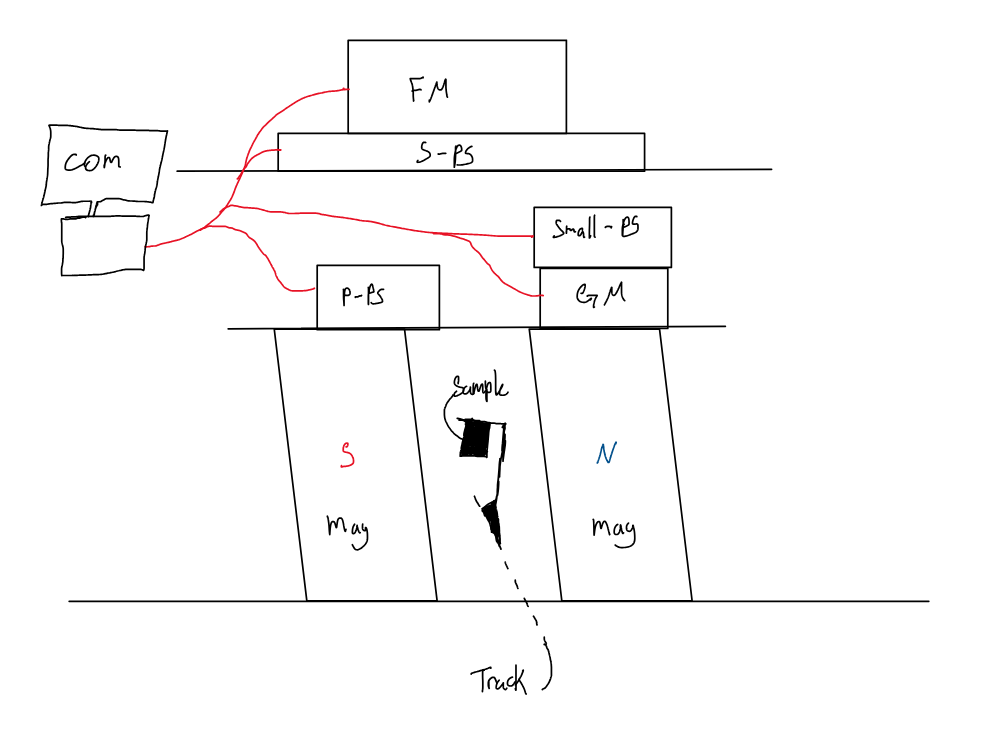
\includegraphics[width=0.8\linewidth]{4-hall_effect/overleaf/images/Screenshot from 2024-10-21 20-48-31.png}
    \caption{ \scriptsize{ Computer (COM), Fluke meter (FM), Sorensen magnet power supply (S-PS), Pasco power supply (P-PS), small power supply for semiconductors (small-PS), Gauss meter (GM), North and South of the hall magnet (N \& S Mag).
    }}
    \label{fig:xray-diagram}
\end{figure}

\begin{multicols}{2}

\section*{Theory \& Procedure}
{
When a current flows in the $+\hat{x}$  direction, the charge carriers flow in the $-\hat{x}$
direction. This flow remains steady in the absence of any external forces. However, when the system is subjected to a magnetic Lorentz force,
\begin{equation}
    \Vec{F}_{mag} = q(\Vec{v} \times \Vec{B})
\end{equation}
the charge carriers experience a vertical deflection. Depending on if the electron or electron-holes carry the charge the Lorentz force will defect the charge carrier according to the direction of ($\Vec{v} \times \Vec{B}$) and the sign on $q$, leading to an accumulation of charge at the vertical edges of the material. This charge imbalance results in a voltage difference across these edges. A multimeter can then be used to measure the magnitude of this voltage difference, as well as determine the sign of the voltage, which indicates whether the charge carriers are electrons or electron-holes. Positive voltage reflects that electron-holes are the carriers and negative voltage reflects that for electrons. 

The vertical component of the magnetic force can be used to determine the Hall coefficient, $R_H$. In the context of this experiment, the relationship is given by:
\begin{equation}
    F_y = E_yh = \Delta V_H = \frac{R_H}{\delta}IB
\end{equation}
where $\delta$ is the thickness of the material and h is the height. But, when considering the Hall voltage between two points, say $a$ \& $b$, a potential difference of IR exist along the sample. Thus the full expression becomes:
\begin{equation}\label{eq:linear_hall}
    \Delta V_{a,b} = \frac{R_H}{\delta}IB + RI
\end{equation}
where R is the resistance of the sample.
 
The first step in initiating this experiment is to ensure that the water pump is activated to cool the Hall magnet, which generates the magnetic field. Next, all equipment—including the power supplies, multimeters, and Gaussmeter—should be powered on. The Sorensen magnet power supply provides current to the magnet's coils and the Pasco power supply maintains a current across the selected sample. The multimeter will be used to measure the voltage across the sample, while the Gaussmeter will measure the strength of the magnetic field passing through the sample.

The next crucial step is to prepare both the software and the sample for measurement. On the computer, we launched the HallScan program, developed in LabView, and set the initial parameters. The magnetic field strength was scanned over a range of 2 to 10 kG (kilogauss), collecting 10 data points. However, for the nickel sample, the number of data points were increased to 15 for enhanced precision. The conductor samples to be scanned include copper (Cu), aluminum (Al), iron (Fe), nickel (Ni), and molybdenum (Mo), each of which were mounted on a holder positioned between the poles of the Hall magnet. The semiconductor samples are silicon (Si) and germanium, Ge-100 and Ge-111. It is important to ensure consistent orientation when mounting the sample and connecting the ± cables. This consistency is crucial for maintaining the same sign on the Hall coefficient throughout the experiment, ensuring reliable and comparable results.
}

\section*{Analysis \& Results}
{
For our data analysis, we opted to convert the data file format sequentially from $.txt$ to $.csv$, and ultimately to $.root$, thereby enabling us to utilize CERN's data analysis tool, ROOT.

We plot the measured Hall voltage ($V_{H}$) against the magnetic field strength ($B_{\text{meas}}$). We anticipated a linear relationship as $B_{\text{meas}}$ approaches infinity. Knowing this we fit data points using ROOT's $\texttt{TF1}$ function and obtain a best-fit slope and y-intercept for each graph.

Before we could further analyze the data, we had to first multiply the best-fit slope by $1 \times 10^{-6}$ to convert the units from [$\frac{\text{mV}}{\text{kG}}$] to [$\frac{\text{V}}{\text{G}}$]. Similarly, for the y-intercept, we multiply by $1 \times 10^{-3}$ to convert from [$\text{mV}$] to [$\text{V}$]. Also, it was important to note that the relationship in Eq.~\eqref{eq:linear_hall} is in slope-intercept form ($y = mx + b$). So, by equating the corresponding terms, we derive Eqs.~\eqref{eq:hall_slope} and \eqref{eq:hall_y}:
\begin{equation}\label{eq:hall_slope}
m = \frac{R_H}{\delta}I \quad \Rightarrow \quad \frac{m\delta}{I}  = R_H
\end{equation}
\begin{equation}\label{eq:hall_y}
b = RI \quad \Rightarrow \quad \frac{b}{I} = R
\end{equation}
From these equations, we use the given thickness of each sample and the current ($I$) measured for each sample to solve these derivations.

For the conductors, measurements were taken at three different currents: 6, 7.5, and 9 Amps. For the semiconductors, measurements were performed at 0.1, 0.5, 1, 5, and 10 Amps.

In Table \ref{tab:hall_hv_resis}, we computed the average Hall coefficient $R_H$ and resistance $R$ for each element at the various currents. The measured values for copper (Cu) and molybdenum (Mo) were reasonably close to the accepted values. However, the measurements for iron (Fe) and nickel (Ni) showed significant deviations from the accepted values and were not within the margin of error, although, they shared the same sign. Based on the sign of the Hall coefficient, we can conclude that electron holes are the charge carriers for Fe and Mo, while electrons are the charge carriers for Cu and Ni.

For semiconductors, the Hall constant and resistance were significantly higher than those observed in the conductors, which is expected due to the intrinsic properties of semiconductors, such as the presence of a band gap. In all the semiconductor samples, electrons can be identified as the charge carriers.

Potential sources of error in this experiment include the calibration of the measurement devices, such as the Fluke meter and Gauss meter, which may not have been perfectly zeroed, leading to propagated inaccuracies in the data. Additionally, inconsistencies in the placement of the sample between the magnet poles may have introduced variability in the magnetic field measurements, further affecting the results.


}

\end{multicols}

\section*{Summary}
{
The experiment aimed to investigate the Hall effect by observing how charge carriers in various materials respond to a magnetic field under different current values. Conductors such as copper, aluminum, iron, nickel, and molybdenum, as well as semiconductors like silicon and germanium, were tested. The Hall voltage was plotted against magnetic field strength and analyzed to calculate the Hall coefficient and resistance for each material. 
}



\begin{table}[]
\centering
\begin{tabular}{c|c|c|c|c|c}
sample & $R_H ({\Omega} cm/G)$  &  $\pm \sigma_{H}$ & accepted $R_H ({\Omega}cm/G)$ & $R$ & $\pm \sigma_{R}$ \\ \hline

Cu & $-3.45E^{-13}$ & $1.28E^{-13}$ & $-0.5E^{-12}$ & $8.18E^{-6}$ & $1.15E^{-7}$ \\
Fe & $5.31E^{-12}$ & $4.98E^{-14}$ & $11E^{-12}$ & $5.31E^{-12}$ & $4.39E^{-7}$ \\
Mo & $1.47E^{-12}$ & $1.13E^{-13}$ & $1.3E^{-12}$ & $-1.12E^{-4}$ & $5.73E^{-7}$ \\
Ni & $-4.43E^{-13}$ & $4.65E^{-13}$ & $-5.1E^{-12}$ & $-4.20E^{-5}$ & $5.30E^{-6}$ \\
Cu-PCB & $-8.81E^{-14}$ & $4.41E^{-15}$ & & $6.06E^{-6}$ & $2.91E^{-7}$ \\
Ge-111 & $-5.46E^{-5}$ & $8.99E^{-5}$ & & $7.89$ & $9.83$ \\
Ge-100 & $-1.38E^{-2}$ & $2.77E^{-2}$ & &  $-3.07E^{2}$ & $5.75E^{2}$ \\
Si & $-2.26E^{-3}$ & $3.39E^{-3}$ & & $1.54E^{1}$ & $2.57E^{1}$ \\
\end{tabular}
\caption{Average Hall coefficient and resistance for currents 6, 7.5, and 9 Amps (for conductors)c- as well as 0.1, 0.5, 1, 5 and 10 Amps for semiconductors}
\label{tab:hall_hv_resis}
\end{table}


\end{document}